%-*- coding: utf-8 -*-
\subsection{Modèle du domaine}
%\rowcolors{2}{Turquoise}{} % {1}{red!26!green!29!blue!31!}{}
\begin{figure}
  \centering
      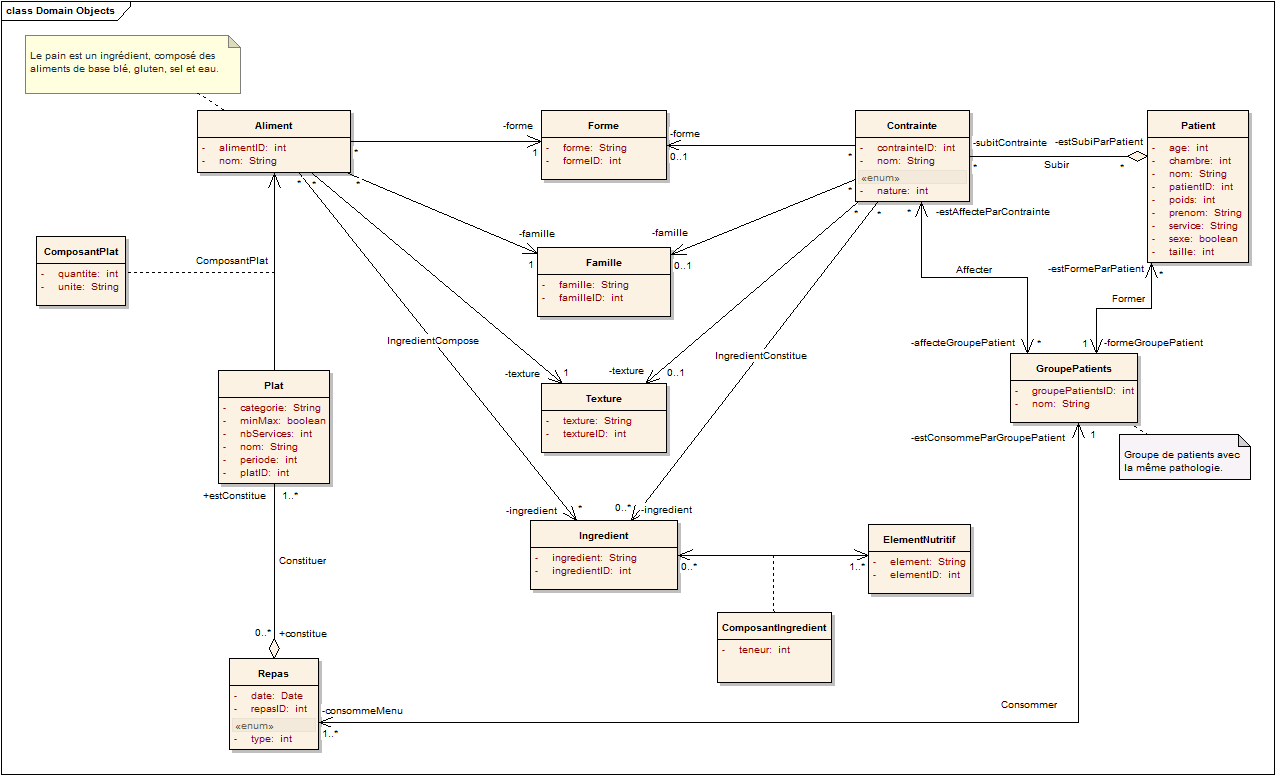
\includegraphics[angle=90, scale=0.55]{../../ModeleDuDomaine/ModeleDuDomaine.png} %
\caption{Modèle du domaine}
\label{ModeleDuDomaine}
\end{figure}

\newcommand{\classe}[1]{\emph{\textbf{#1}}}
\newcommand{\attribut}[1]{\emph{#1}}
\newcommand{\regleD}[1]{\textcolor{NavyBlue}{#1}}
\newcommand{\regleT}[1]{\textcolor{ForestGreen}{#1}}

Le modèle du domaine est représenté \autoref{ModeleDuDomaine}. Ce projet ayant pour objet l'alimentation des personnes hospitalisées, nous considérons les pathologies de ces personnes sous l'aspect de leur impact sur le plan alimentaire, et pour être plus précis sur les aliments qui s'avéreraient être interdits à cause de telle ou telle pathologie. Ces pathologies constituant des contraintes sur le plan alimentaire, c'est la classe \classe{Contrainte} qui les décrit. Elle a un attribut \attribut{nom} pour la désigner, un attribut \attribut{nature} qui permet de déterminer s'il sagit d'une allergie
\footnote{\label{allergies}\href{https://allergies.afpral.fr/allergie/en-savoir-plus-sur-les-allergies/alimentaires/89-liste-des-14-allergenes-alimentaires-majeurs}{AFPRAL: Liste des 14 allergènes alimentaires majeurs.}},
d'une contre~indications
\footnote{\label{contreIndications}La prise de certains médicaments interdit la consommation de certains aliments.}
ou d'une maladie.
Les contraintes peuvent porter aussi bien sur l'aliment luis même, que sur sa forme (solide, liquide), sa famille (fruits à coque, crustacès, ...) ou sa texture
\footnote{\label{textures}Terme métier pour dire si l'on travaille avec des \href{http://plone.vermeil.org:8080/ehpad/Bibliotheque/Memoires/annee-2012-2013/07 - Les textures modifiees et le plaisir de manger de Jacques Caby.pdf}{aliments à texture modifiée} (mixés) ou à texture maintenue (entiers).}.
Les quatres classes \classe{Ingredient}, \classe{Forme}, \classe{Famille} et \classe{Texture} véhicules ces informations. Elles servent aussi à renseigner la classe \classe{Aliment} qui définit les alimentss composant un \classe{Plat}. Les quantités misent en oeuvre sont décrites dans la classe~association \classe{ComposantPlat}. Un plat, en plus des aliments qui le composent, contient des informations liées à sa fréquence de service: nombre de services (\attribut{nbServices}) maximum ou minimum (\attribut{minMax}) par période (\attribut{periode}).
La classe \classe{GroupePatients} permet d'avoir la liste des patients qui subissent les mêmes contraintes alimentaires. Il y aura donc autant de menus à faire qu'il y a de groupes de patients.

\subsection{Modèle Logique de Données}
Le dictionnaire est décrit \autoref{DictionnaireMDD}.
\begin{description}
\item[Règle 1:] classe = relation, si héritage, les classes filles contiennent l'identifiant de la classe mère comme clè étrangère.
\regleD{\item[Règle 2:] association 1 à plusieurs devient clé étrangère de la classe fille}
\regleT{\item[Règle 3:] association plusieurs à plusieurs devient relation avec clé primaire composé des 2 clé primaires des 2 classes en relations.}
\end{description}

Aliment(\underline{alimentID}, nom, \regleD{famille\#}, \regleD{texture\#}, \regleD{forme\#})

\regleT{ComposantPlat(\underline{alimentID\#, platID\#}, quantite, unite)}

Plat(\underline{platID}, nom, categorie, nbServices, periode, minMax)

\regleT{Constituer(\underline{repasID\#, platID\#})}

Repas(\underline{repasID}, date, type, \regleD{groupePatientsID\#})

Patient(\underline{patientID}, prenom, nom, sexe, age, poids, taille, service, chambre, \regleD{groupePatientsID\#})

\regleT{Subir(\underline{patientID\#, contrainteID\#})}

Contrainte(\underline{contrainteID}, nom, nature, \regleD{famille\#}, \regleD{texture\#}, \regleD{forme\#})

\regleT{Affecter(\underline{groupePatientsID\#, contrainteID\#})}

GroupePatients(\underline{groupePatientsID}, nom)

Formes(\underline{formeID}, forme)

Familles(\underline{familleID}, famille)

Textures(\underline{textureID}, texture)

Ingredient(\underline{ingredientID}, ingredient)

\regleT{IngredientCompose(\underline{alimentID\#, ingredientID\#})}

\regleT{IngredientConstitue(\underline{contrainteID\#, ingredientID\#})}

ElementNutritif(\underline{elementID}, element)

\regleT{ComposantIngredient(\underline{elementID\#, ingredientID\#}, teneur)}

\begin{longtable}{llp{5cm}ll}
  \hline
  \textbf{Classe} & \textbf{Attribut} & \textbf{Description} & \textbf{Type} & \textbf{Contrainte} \\ \endfirsthead \hline
  \textbf{Classe} & \textbf{Attribut} & \textbf{Description} & \textbf{Type} & \textbf{Contrainte} \\ \endhead \hline
  Aliment & alimentID & Clé primaire & Integer & Identifiant \\
  Aliment & nom & Nom de l'aliment & String & \\
  Aliment & famille & Clé étrangère & Integer & \\
  Aliment & texture & Clé étrangère & Integer & \\
  Aliment & forme & Clé étrangère & Integer & \\ \hline
  ComposantPlat & alimentID & Clé étrangère & Integer & Identifiant \\
  ComposantPlat & platID & Clé étrangère & Integer & Identifiant \\
  ComposantPlat & quantite & Quantité d'ingrédient dans le plat & Integer & \\
  ComposantPlat & unite & Unité de mesure de la quantité & String & \\ \hline
  Plat & platID & Clé primaire & Integer & Identifiant \\
  Plat & nom & Nom du plat & String & \\
  Plat & categorie & Entrée, plat, dessert, petit déjeuner & String & \\
  Plat & nbServices & Fréquence de service & Integer & \\
  Plat & periode & Période de la fréquence de service & Integer & \\
  Plat & minMax & Fréquence de service min ou max & Boolean & \\ \hline
  Constituer & repasID & Clé étrangère & Integer & Identifiant \\
  Constituer & platID & Clé étrangère & Integer & Identifiant \\ \hline
  Repas & repasID & Clé primaire & Integer & Identifiant \\
  Repas & date & Date du repas & Date &  \\
  Repas & type & Petit déjeuner, déjeuner, diner & Integer \\
  Repas & groupePatientID &  Groupe de patients auxquels est destiné le repas & Integer & Clé étrangère \\ \hline
  Patient & patientID & Clé primaire & Integer & Identifiant \\
  Patient & prenom & Prénom du patient & String & Non NULL\\
  Patient & nom & Nom du patient & String & Non NULL\\
  Patient & sexe & Sexe du patient & Boolean & \\
  Patient & age & Age du patient & Integer & $\geqslant 18$\\ %
  Patient & poids & Poids du patient & Integer & $> 0$ \\
  Patient & taille & Taille du patient & Integer & $> 0$ \\
  Patient & service & Service dans lequel ce trouve le patient & String & \\
  Patient & chambre & Numéro de chambre du patient & Integer & $> 0$ \\
  Patient & groupePatientID &  Groupe de patients auquels auquel apartient le patient & Integer & Clé étrangère \\ \hline
  Subir & patientID & Clé étrangère & Integer & Identifiant \\
  Subir & contrainteID & Clé étrangère & Integer & Identifiant \\ \hline
  Contrainte & contrainteID & Clé primaire & Integer & Identifiant \\
  Contrainte & nom & Nom de la contrainte & String & Non NULL \\
  Contrainte & nature & Nature de la contrainte & Natures & \\
  Contrainte & famille & Famille de l'aliment & Familles & \\
  Contrainte & texture & Texture de l'aliment & Textures & \\
  Contrainte & forme & Forme de l'aliment & Formes & \\ \hline
  Affecter & groupePatientsID & Clé étrangère & Integer & Identifiant \\
  Affecter & contrainteID & Clé étrangère & Integer & Identifiant \\ \hline
  GroupePatients & groupePatientsID & Clé primaire & Integer & Identifiant \\
  GroupePatients & nom & Nom du groupe de patients & String & \\ \hline
  Formes & formeID & Clé primaire & Integer & Identifiant \\
  Formes & forme & Forme de l'aliment & String & \\ \hline
  Familles & familleID & Clé primaire & Integer & Identifiant \\
  Familles & famille & Famille de l'aliment & String & \\ \hline
  Textures & textureID & Clé primaire & Integer & Identifiant \\
  Textures & texture & Texture de l'aliment & String & \\ \hline
  Ingredient & ingredientID & Clé primaire & Integer & Identifiant \\
  Ingredient & ingredient & Nom de l'ingrédient & String &  \\ \hline
  IngredientCompose & alimentID & Clé étrangère & Integer & Identifiant \\
  IngredientCompose & ingredientID & Clé étrangère & Integer & Identifiant \\ \hline
  IngredientConstitue & ingredientID & Clé étrangère & Integer & Identifiant \\
  IngredientConstitue & contrainteID & Clé étrangère & Integer & Identifiant \\ \hline
  ComposantIngredient & ingredientID & Clé étrangère & Integer & Identifiant \\
  ComposantIngredient & elementID & Clé étrangère & Integer & Identifiant \\
  ComposantIngredient & teneur & Teneur d'élément nutritif dans un ingrédient (\%) & Integer & \\ \hline
  ElementNutritif & elementID & Clé primaire & Integer & Identifiant \\
  ElementNutritif & element & Nomd de l'élément & String &  \\ \hline
\caption{Dictionnaire}
\label{DictionnaireMDD}
\end{longtable}

%\hiderowcolors
